% Section 6: Resultats i Discussió (fusió d'Experiments + Discussió)

\section{Resultats i Discussió}
\label{sec:resultats}

\subsection{Configuració experimental}

Tots els experiments s'han executat amb Python 3.9, InterpretML 0.4.3, scikit-learn 1.2.0, validació creuada de 5 folds (seed=42) sobre un dataset de \textbf{956 mostres i 56 variables}. Les mètriques emprades són MAE (Mean Absolute Error), RMSE (Root Mean Squared Error) i R² (Coefficient of Determination), calculades amb mitjana i desviació estàndard per avaluar estabilitat.

\subsection{Resultats quantitatius i millora progressiva}

La Taula~\ref{tab:progressive_improvement} mostra la millora progressiva des del model baseline Lasso fins a la millor configuració de Fase 4, demostrant l'efectivitat de la metodologia proposada.

\begin{table}[htbp]
\centering
\caption{Evolució progressiva del rendiment del model a través de les fases de la metodologia.}
\label{tab:progressive_improvement}
\scriptsize
\resizebox{\columnwidth}{!}{%
\begin{tabular}{@{}lrrr@{}}
\toprule
\textbf{Fase} & \textbf{MAE} & \textbf{RMSE} & \textbf{R²} \\
\midrule
Lasso (Baseline) & 1.126 & 1.646 & 0.332 \\
EBM Fase 1 & 1.072 & 1.602 & 0.368 \\
EBM Fase 3 & 1.018 & 1.466 & 0.470 \\
\textbf{EBM Fase 4 (Robust)} & \textbf{0.950} & \textbf{1.368} & \textbf{0.422} \\
\midrule
\textbf{Millora total (\%)} & \textbf{-15.6\%} & \textbf{-16.9\%} & \textbf{+27.1\%} \\
\bottomrule
\end{tabular}%
}
\end{table}

S'ha aconseguit una reducció del \textbf{15.6\% en MAE} i del \textbf{16.9\% en RMSE}, amb increment del 27.1\% en R². Cal destacar que la Fase 3 obté un R² superior (0.470) però amb menys estabilitat. La configuració \textbf{Robust (Leaf=10)} de Fase 4 ofereix el millor compromís entre precisió i robustesa: MAE = 0.950, RMSE = 1.368, R² = 0.422, amb desviacions estàndard contingudes que garanteixen estabilitat entre folds. Aquesta robustesa és crítica per a aplicació industrial, on la fiabilitat és tan important com la precisió puntual.

\subsection{Comparació de configuracions en Fase 4}

S'han avaluat set configuracions d'EBM en Fase 4, explorant diferents compromisos entre precisió, interpretabilitat i robustesa. La Taula~\ref{tab:phase4_results} mostra els resultats.

\begin{table}[htbp]
\centering
\caption{Resultats de les set configuracions d'EBM en Fase 4 amb 5-fold cross-validation.}
\label{tab:phase4_results}
\scriptsize
\resizebox{\columnwidth}{!}{%
\begin{tabular}{@{}lrrr@{}}
\toprule
\textbf{Configuració} & \textbf{MAE} $\pm$ std & \textbf{RMSE} $\pm$ std & \textbf{R²} $\pm$ std \\
\midrule
\textbf{Robust (Leaf=10)} & \textbf{0.950 $\pm$ 0.063} & \textbf{1.368 $\pm$ 0.153} & \textbf{0.422 $\pm$ 0.109} \\
High Interactions (25) & 0.953 $\pm$ 0.057 & 1.370 $\pm$ 0.136 & 0.421 $\pm$ 0.094 \\
Current Best & 0.953 $\pm$ 0.060 & 1.371 $\pm$ 0.154 & 0.420 $\pm$ 0.107 \\
High Precision (512 bins) & 0.954 $\pm$ 0.059 & 1.371 $\pm$ 0.149 & 0.420 $\pm$ 0.103 \\
Slow/Deep Learning & 0.954 $\pm$ 0.068 & 1.381 $\pm$ 0.155 & 0.412 $\pm$ 0.105 \\
Smooth Sensors (128 bins) & 0.956 $\pm$ 0.059 & 1.378 $\pm$ 0.149 & 0.415 $\pm$ 0.101 \\
Simple/Stable & 0.963 $\pm$ 0.069 & 1.411 $\pm$ 0.162 & 0.387 $\pm$ 0.108 \\
\bottomrule
\end{tabular}%
}
\end{table}

Les configuracions amb més regularització (Robust, Current Best) superen les més complexes, confirmant que amb datasets limitats (956 mostres) la simplificació del model és més beneficiosa que l'increment de capacitat representacional.

\subsection{Comparació amb models alternatius}
\label{subsec:comparacio_models_alternatius}

Un dels interrogants clau d'aquest treball és si la restricció d'interpretabilitat penalitza el rendiment predictiu. A diferència de les Taules~\ref{tab:progressive_improvement} i~\ref{tab:phase4_results}, que utilitzen validació creuada de 5 folds, els resultats d'aquesta secció corresponen al conjunt de test fix (242 mostres, 25\% del dataset) per garantir comparabilitat directa entre models amb arquitectures heterogènies. S'ha comparat el model proposat (EBM filter+interact) amb quatre alternatives representatives: (A) LASSO com a referència lineal, (B) EBM sense filtratge previ per aïllar l'efecte de la fase de \emph{pruning}, (C) XGBoost optimitzat amb GridSearchCV (48 combinacions d'hiperparàmetres) com a representant \emph{black-box}, i (D) LASSO+EBM per avaluar si la selecció lineal de variables és adequada per a models no lineals.

\begin{table}[htbp]
\centering
\caption{Benchmark comparatiu de 5 models (test set, 242 mostres).}
\label{tab:model_comparison}
\scriptsize
\resizebox{\columnwidth}{!}{%
\begin{tabular}{@{}lrrrr@{}}
\toprule
\textbf{Model} & \textbf{MAE} & \textbf{R²} & \textbf{Termes} & \textbf{Train (s)} \\
\midrule
\textbf{EBM filter+interact} & \textbf{0.994} & \textbf{0.477} & 25 & 4.9 \\
EBM full (no filter) & 1.026 & 0.395 & 66 & 11.6 \\
LASSO (full) & 1.038 & 0.383 & 36 & 0.1 \\
XGBoost tuned & 1.037 & 0.369 & 2500 & 78.2 \\
LASSO + EBM & 1.177 & 0.202 & 18 & 4.3 \\
\bottomrule
\end{tabular}%
}
\end{table}

Els resultats (Taula~\ref{tab:model_comparison} i Figura~\ref{fig:model_comparison}) demostren tres conclusions operativament rellevants:

\textbf{(1) La interpretabilitat no penalitza el rendiment.} L'EBM filter+interact supera XGBoost en R² per un marge del 29\% relatiu (0.477 vs 0.369), invalidant l'assumpció habitual que els models \emph{glass-box} sacrifiquen precisió per guanyar transparència. En el context GxP, on cada predicció ha de ser justificable davant auditoria \cite{gamp5}, aquest resultat elimina la tensió entre compliment normatiu i capacitat analítica.

\textbf{(2) El filtratge de característiques és l'element diferencial.} La comparació directa entre EBM amb i sense filtratge (R²: 0.477 vs 0.395, p=0.037 en test de Wilcoxon) demostra que reduir de 56 a 15 variables no perd informació sinó que elimina soroll que degrada la capacitat de generalització. Amb 956 mostres, l'espai d'interaccions de 56 variables ($\binom{56}{2}$=1.540 parells possibles) excedeix la capacitat d'estimació fiable; reduint a 15 variables ($\binom{15}{2}$=105 parells) es garanteix densitat de dades suficient per interacció.

\textbf{(3) La selecció lineal de variables és inadequada per a models no lineals.} El model LASSO+EBM (R² = 0.202) obté el pitjor resultat, evidenciant que LASSO descarta variables amb efectes no lineals importants que l'EBM sí aprofita quan les selecciona pel seu propi criteri d'importància.

\begin{figure}[htbp]
    \centering
    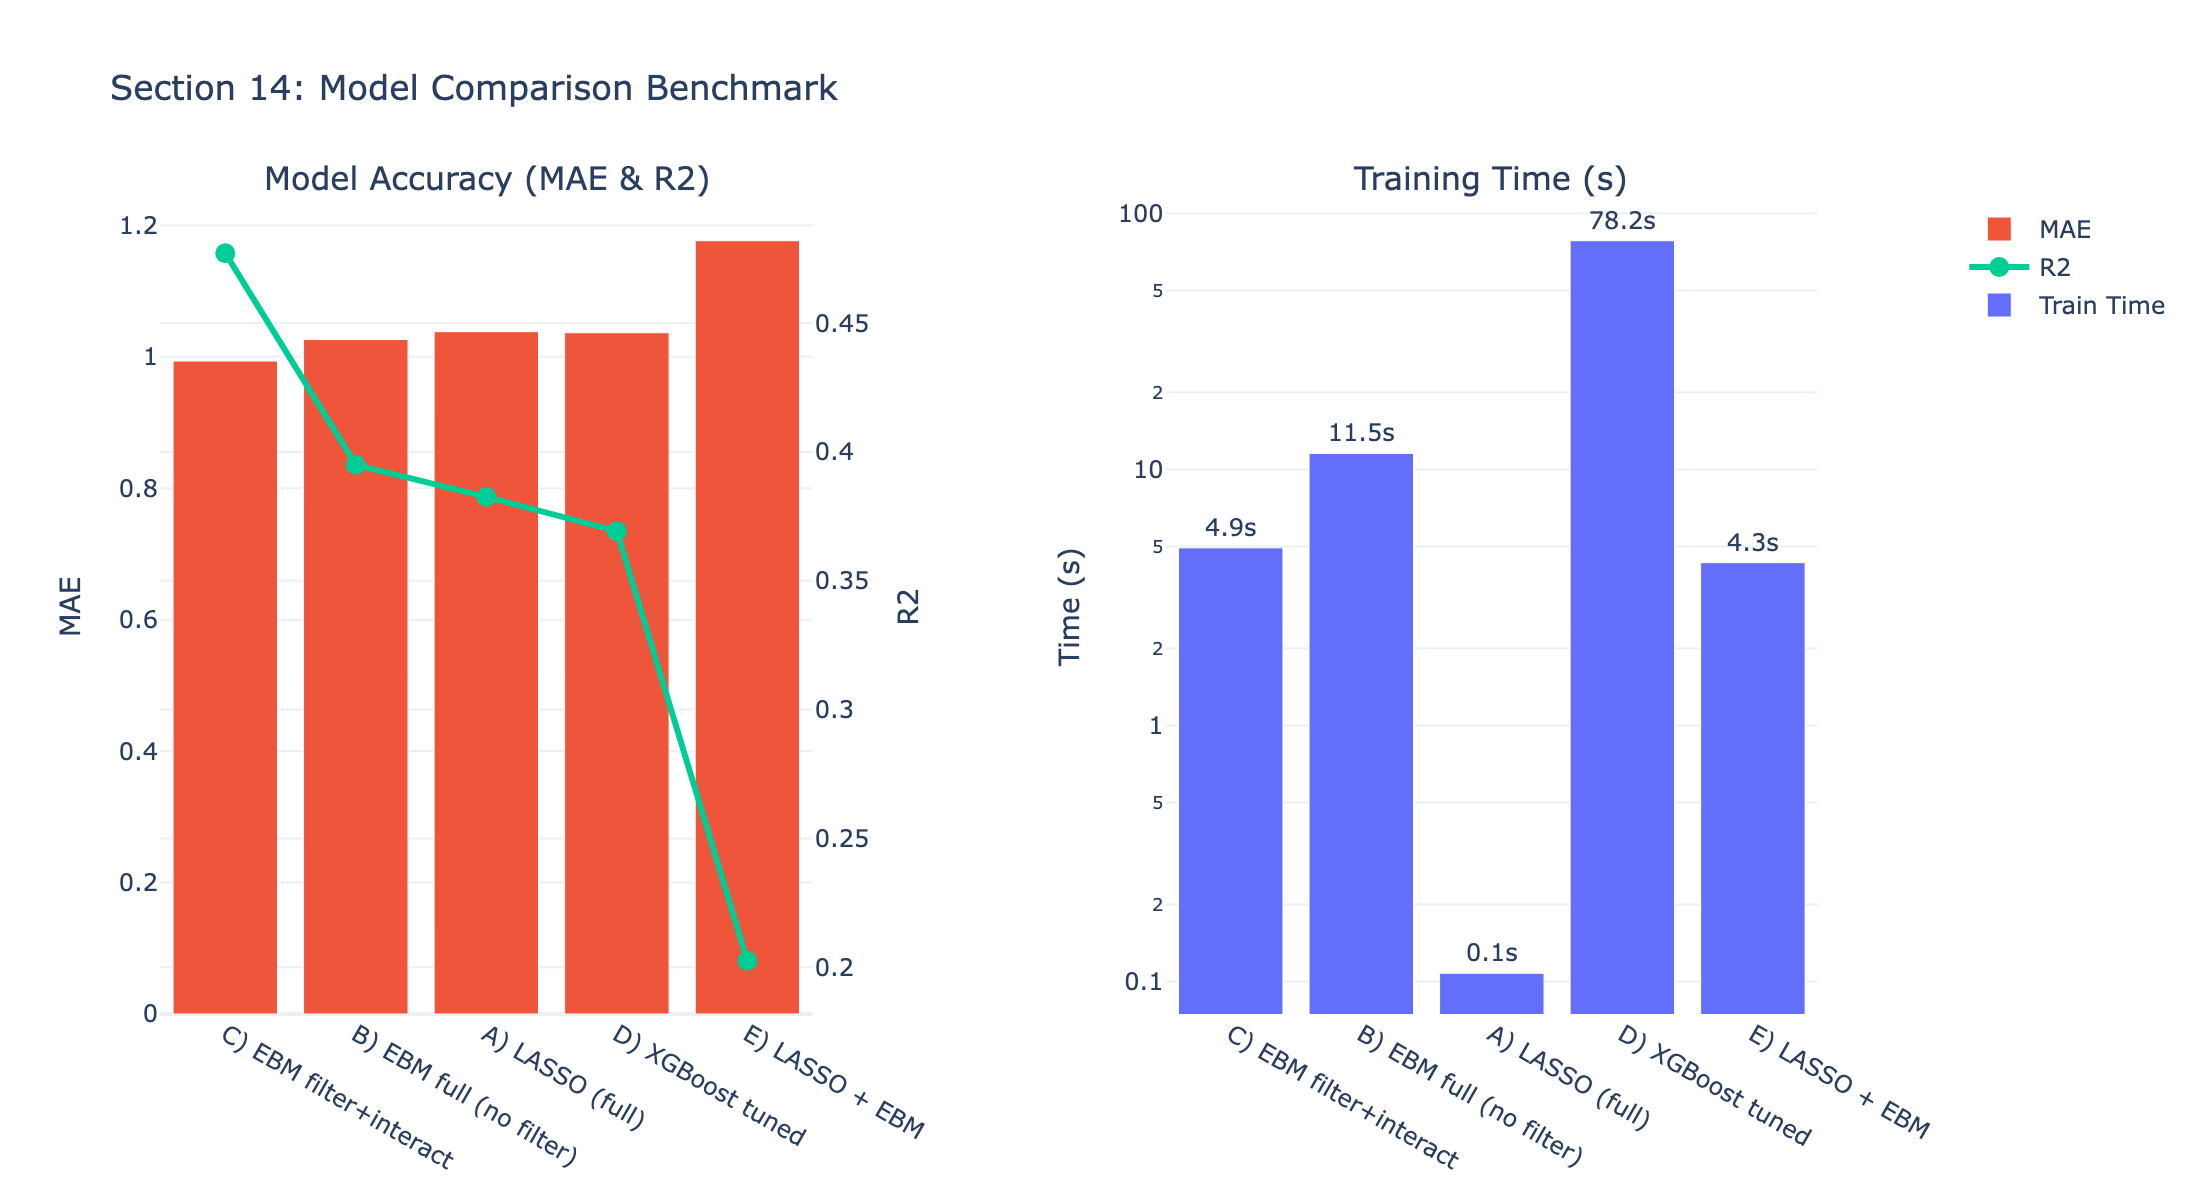
\includegraphics[width=\columnwidth]{images/s14_model_comparison.png}
    \caption{Comparació de rendiment (MAE, R²) i temps d'entrenament dels 5 models avaluats.}
    \label{fig:model_comparison}
\end{figure}

La Figura~\ref{fig:complexity_vs_r2} condensa l'argument central d'aquest treball: el model proposat ocupa la posició òptima a l'espai complexitat-rendiment. Amb només 25 termes interpretables (15 efectes principals + 10 interaccions), supera en R² un XGBoost amb 2.500 paràmetres estimats. Aquesta diferència de dos ordres de magnitud en complexitat té implicacions directes: cada terme del model EBM pot ser revisat, validat i justificat per un enginyer de procés en menys d'una hora, mentre que un XGBoost requereix tècniques post-hoc (SHAP) que afegeixen una capa d'aproximació i incertesa interpretativa \cite{rudin2021fundamental}.

\begin{figure}[htbp]
    \centering
    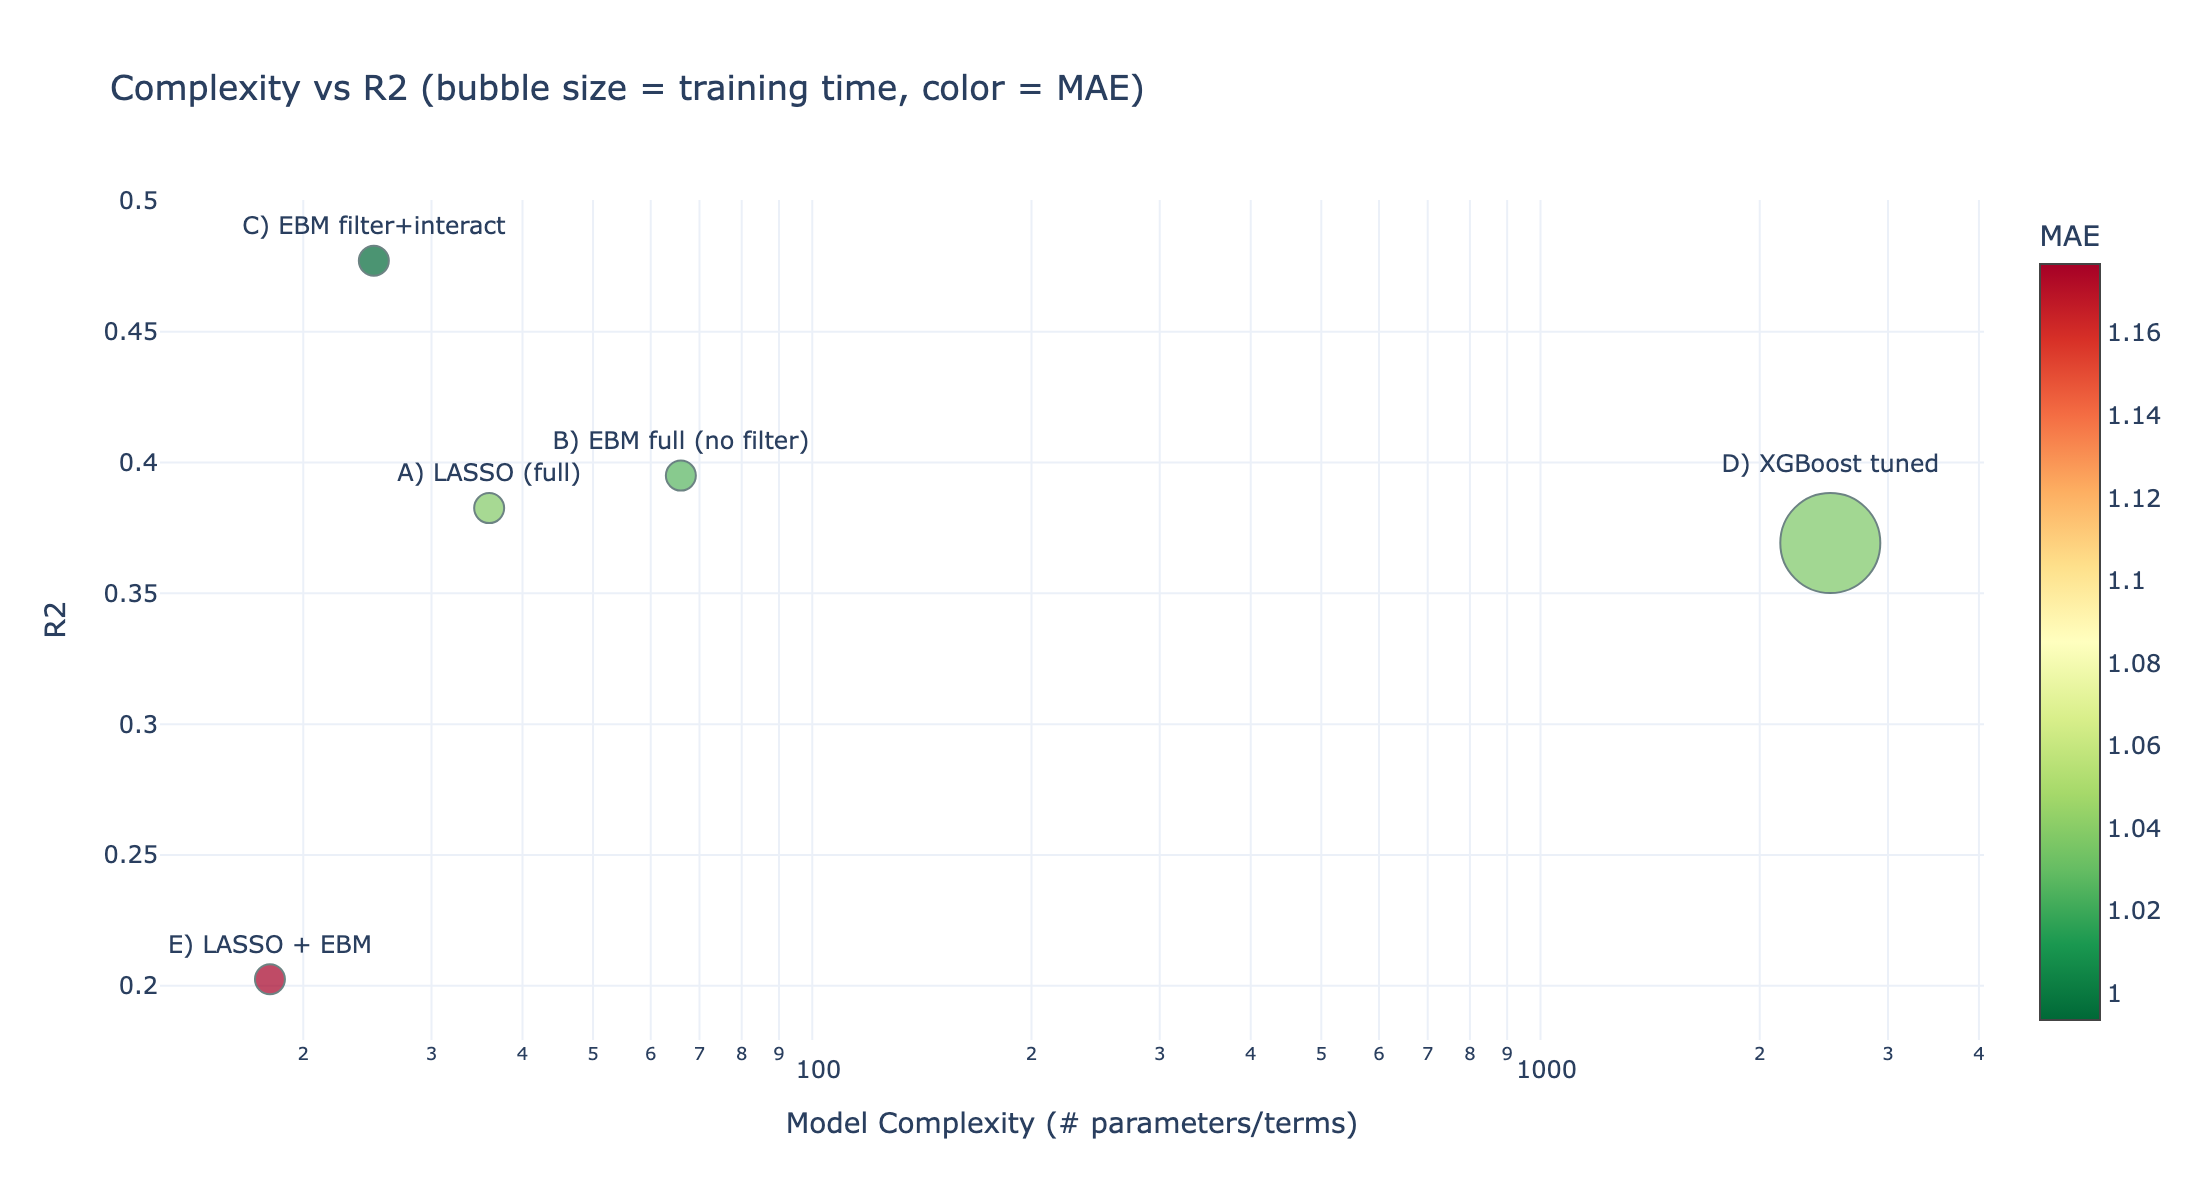
\includegraphics[width=\columnwidth]{images/s14_complexity_vs_r2.png}
    \caption{Compromís complexitat-rendiment: nombre de termes/paràmetres (eix x, escala log) vs R² (eix y). La mida de la bombolla codifica temps d'entrenament i el color, MAE.}
    \label{fig:complexity_vs_r2}
\end{figure}

\subsection{Viabilitat computacional per a industrialització}
\label{subsec:viabilitat_computacional}

La viabilitat d'un sistema RCA en producció no depèn únicament de la precisió predictiva, sinó de la seva capacitat d'operar dins dels requisits temporals del procés. En el context de fraccionament de plasma, on cada lot genera dades finals en un cicle de 24-48h i la presa de decisions ha de ser quasi-immediata per evitar propagació de desviacions, el model ha de complir dos requisits: (1) inferència en temps real per alimentar dashboards operatius, i (2) reentrenament ràpid per adaptar-se a canvis de procés sense aturar el sistema.

\begin{figure}[htbp]
    \centering
    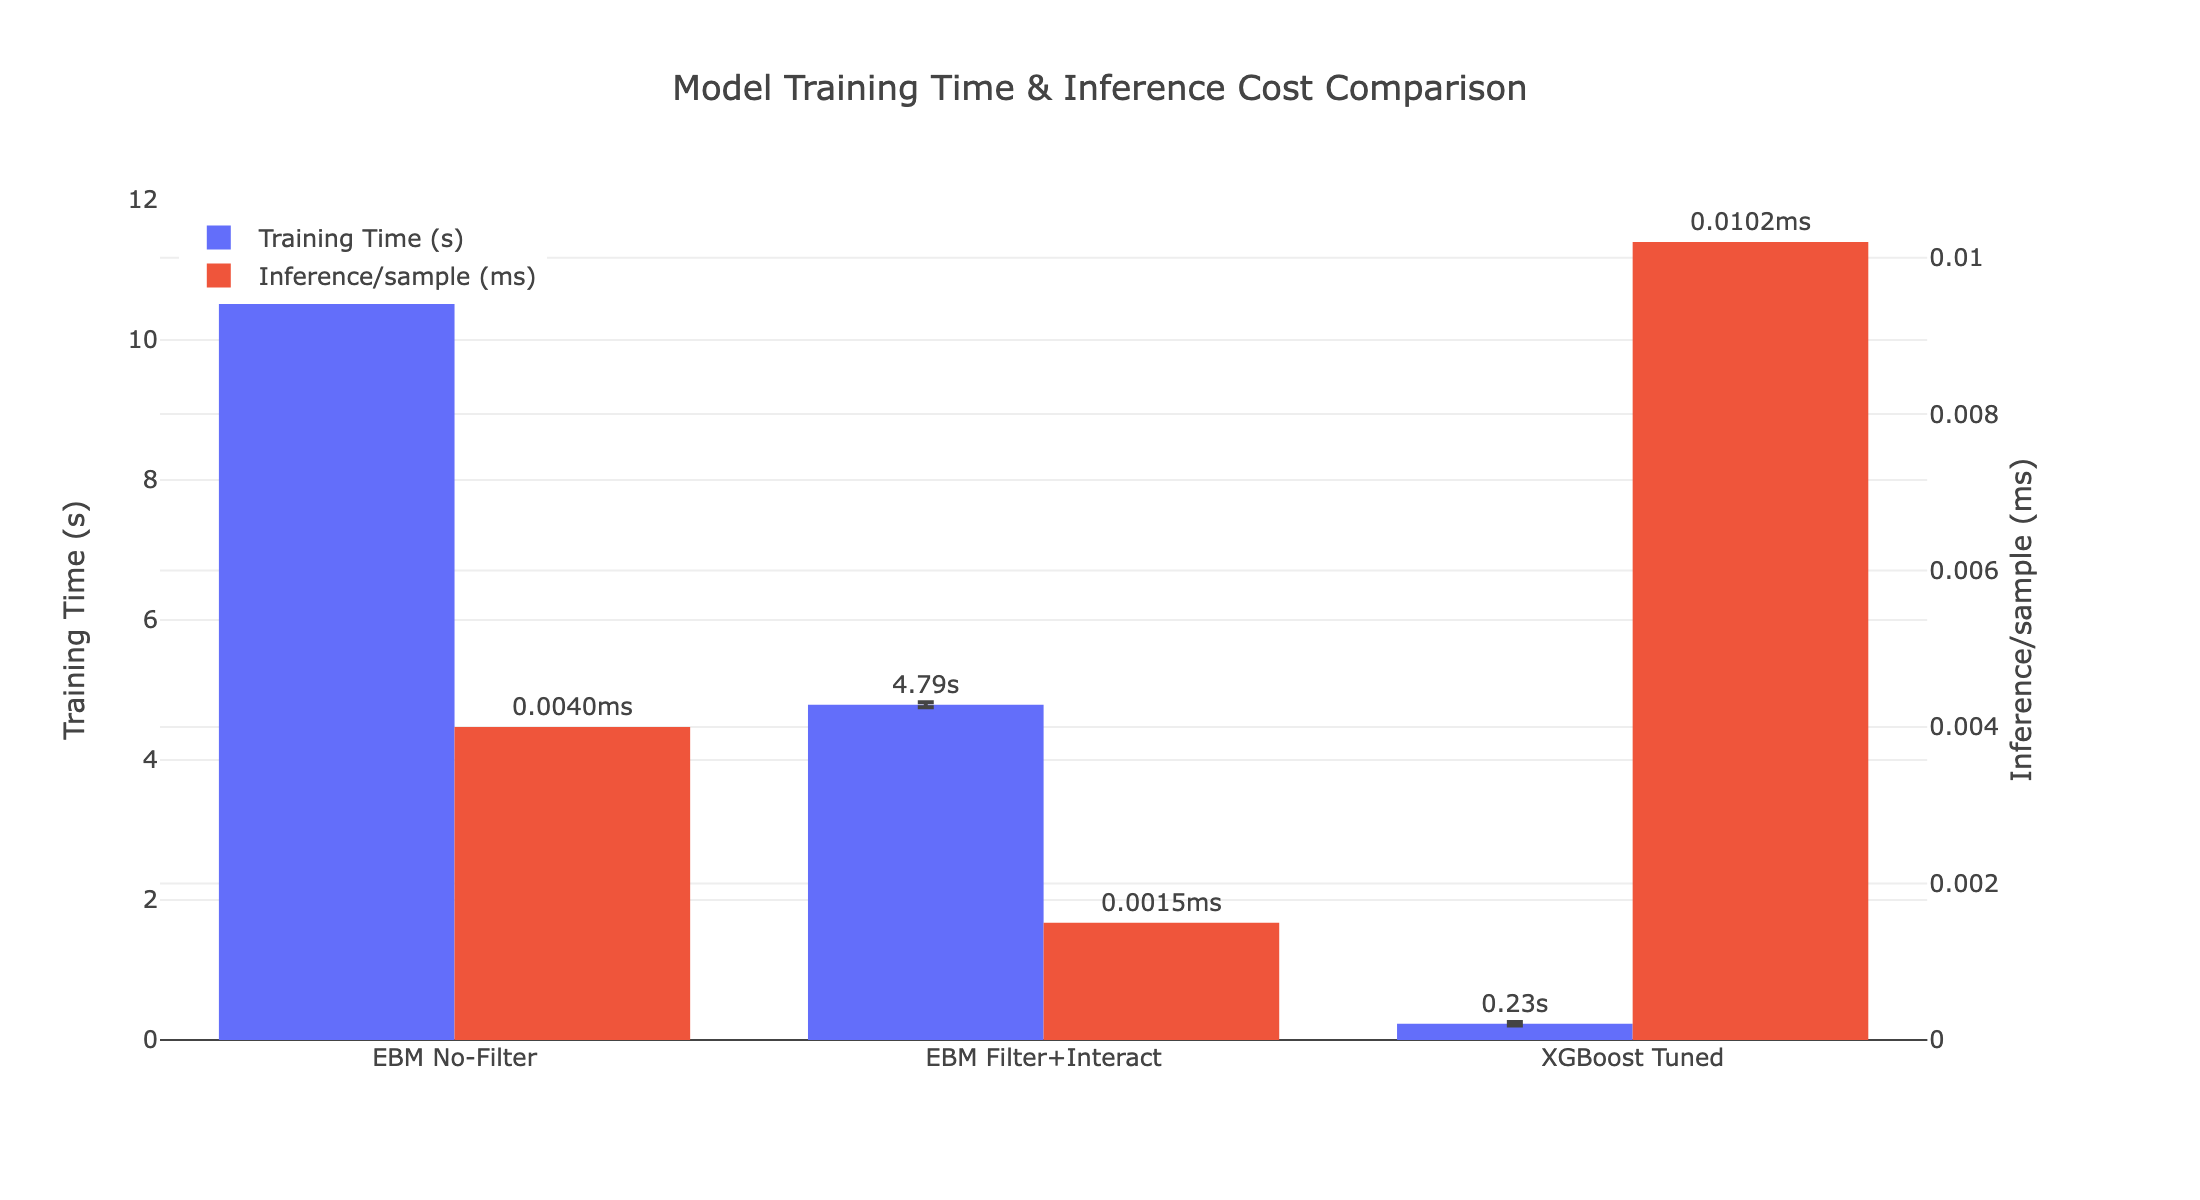
\includegraphics[width=\columnwidth]{images/s15_training_inference_cost.png}
    \caption{Comparació de temps d'entrenament i latència d'inferència entre EBM (amb i sense filtratge) i XGBoost.}
    \label{fig:training_inference_cost}
\end{figure}

La Figura~\ref{fig:training_inference_cost} i la Taula~\ref{tab:computational_viability} demostren que el model proposat compleix ambdós requisits amb marge ampli.

\begin{table}[htbp]
\centering
\caption{Comparació de cost computacional entre models.}
\label{tab:computational_viability}
\scriptsize
\resizebox{\columnwidth}{!}{%
\begin{tabular}{@{}lrrr@{}}
\toprule
\textbf{Mètrica} & \textbf{EBM filter} & \textbf{EBM no-filter} & \textbf{XGBoost} \\
\midrule
Temps entrenament (s) & \textbf{4.8} & 11.4 & 78.2 \\
Latència inferència (ms/mostra) & \textbf{0.0015} & 0.0040 & 0.0102 \\
Throughput (batches/s) & \textbf{688.000} & 248.000 & 99.000 \\
Empremta model (MB) & 2.7 & 4.1 & 0.5 \\
\bottomrule
\end{tabular}%
}
\end{table}

El model proposat aconsegueix la menor latència (0.0015~ms/mostra, equivalent a 688.000 prediccions/segon), permetent processar la totalitat de la producció anual (aprox. 1.000 lots) en menys de 2~ms i la integració directa amb sistemes MES/SCADA sense impacte en els temps de cicle. El temps de reentrenament de 4.8~s habilita una estratègia de reentrenament per lot sense requerir infraestructura de computació dedicada, i l'empremta de 2.7~MB permet desplegament en contenidors lleugers sense GPU, compatible amb arquitectures \emph{edge} en planta.

Des d'una perspectiva de cost operatiu, la combinació de latència mínima i reentrenament ràpid permet desplegar el sistema com a servei continu sense \emph{batch scheduling}, reduint la complexitat d'infraestructura IT i els costos associats de manteniment.

\subsection{Monitoratge retrospectiu de drift}
\label{subsec:monitoratge_drift}

Un model desplegat en producció perd validesa quan les distribucions de les variables d'entrada canvien respecte a les condicions d'entrenament. Per quantificar aquest risc de manera prospectiva, s'ha implementat un sistema de monitoratge basat en el \emph{Population Stability Index} (PSI) sobre finestres lliscants de 50 lots amb pas de 25, avaluant les 5 variables de major importància del model.

La Figura~\ref{fig:drift_psi} mostra els resultats del monitoratge retrospectiu sobre les darreres 290 mostres (30\% del dataset, cronològicament ordenades):

\begin{figure}[htbp]
    \centering
    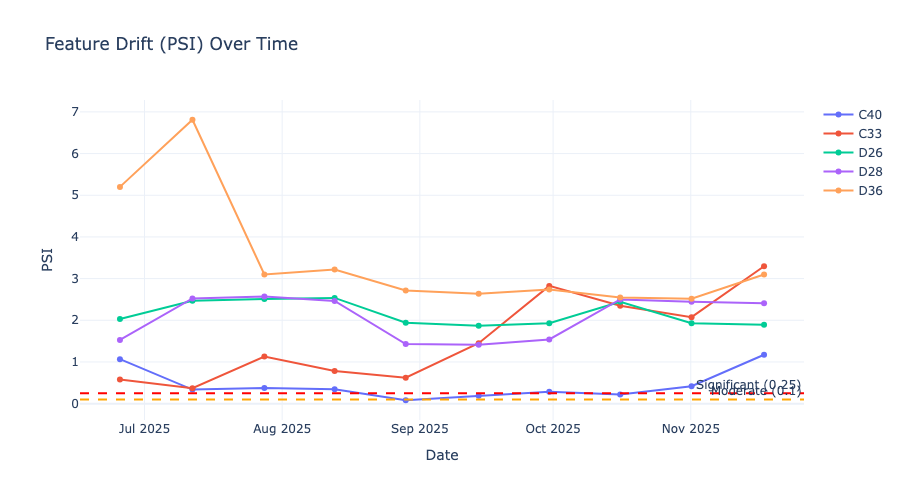
\includegraphics[width=\columnwidth]{images/drift.png}
    \caption{Evolució del PSI per a les 5 variables principals del model. Línia discontínua vermella: llindar de drift significatiu (PSI $>$ 0.25).}
    \label{fig:drift_psi}
\end{figure}

L'anàlisi revela un patró de drift generalitzat des de juny 2025, amb dues observacions críticament rellevants per a la industrialització:

\textbf{(1) Drift extrem en variables de filtració.} D36 (nombre total de papers gruixuts) assoleix PSI=6.8, indicant un canvi radical en la distribució d'aquesta variable — probablement un canvi de material o protocol de filtració. Aquesta magnitud de drift (PSI $>$ 5 és considerat crític en la literatura \cite{lu2020drift}) implica que les shape functions apreses per D36 operen fora del rang d'entrenament, comprometent potencialment la fiabilitat de les contribucions locals.

\textbf{(2) Robustesa del model malgrat el drift.} Malgrat els valors extrems de PSI, el MAE del model sobre les finestres d'avaluació es manté per sota del límit de control superior (UCL=2.55) en totes les finestres. Això demostra que l'estructura additiva de l'EBM proporciona una degradació gradual: quan una variable deriva, les restants 14 variables i 10 interaccions mantenen capacitat predictiva. Tanmateix, la recomanació operativa és activar reentrenament quan qualsevol variable superi PSI $>$ 0.25 durant 3 finestres consecutives, per prevenir acumulació de biaix.

Aquesta anàlisi valida empíricament la necessitat de la capa de monitoratge proposada a la Secció~\ref{subsec:capa_validacio_industrialitzacio} i demostra que el sistema detecta proactivament condicions que requereixen intervenció, abans que es tradueixin en degradació mesurable del rendiment predictiu.

\subsection{Interpretació dels resultats i utilitat per a RCA}

L'anàlisi mostra que el guany predictiu prové de la combinació d'efectes principals i interaccions rellevants, no d'una única variable dominant. Els factors més crítics identificats inclouen variables de condicions de tanc, temps de mescla, configuracions de filtració i estructura operativa del lot. Les interaccions més rellevants combinen variables de preparació i filtració, explicant comportaments no lineals impossibles de captar amb models lineals.

\subsubsection{Avantatge de la interpretabilitat nativa: shape functions vs SHAP}

La Figura~\ref{fig:shape_c33} il·lustra un cas paradigmàtic de la superioritat interpretativa de l'EBM respecte a models \emph{black-box} amb explicabilitat post-hoc. La variable C33 (temps total de mescla de Fracció I) exhibeix una relació fortament no lineal amb el yield D49: el punt òptim se situa a 3.04 minuts (+0.276 punts percentuals de contribució), amb un rang segur entre 1.2 i 9.3 minuts on l'impacte és positiu o neutre. Més enllà de 10 minuts, la penalització creix de manera progressiva fins a $-$0.6~pp per a valors superiors a 35 minuts — un patró de saturació que cap model lineal pot capturar.

\begin{figure}[htbp]
    \centering
    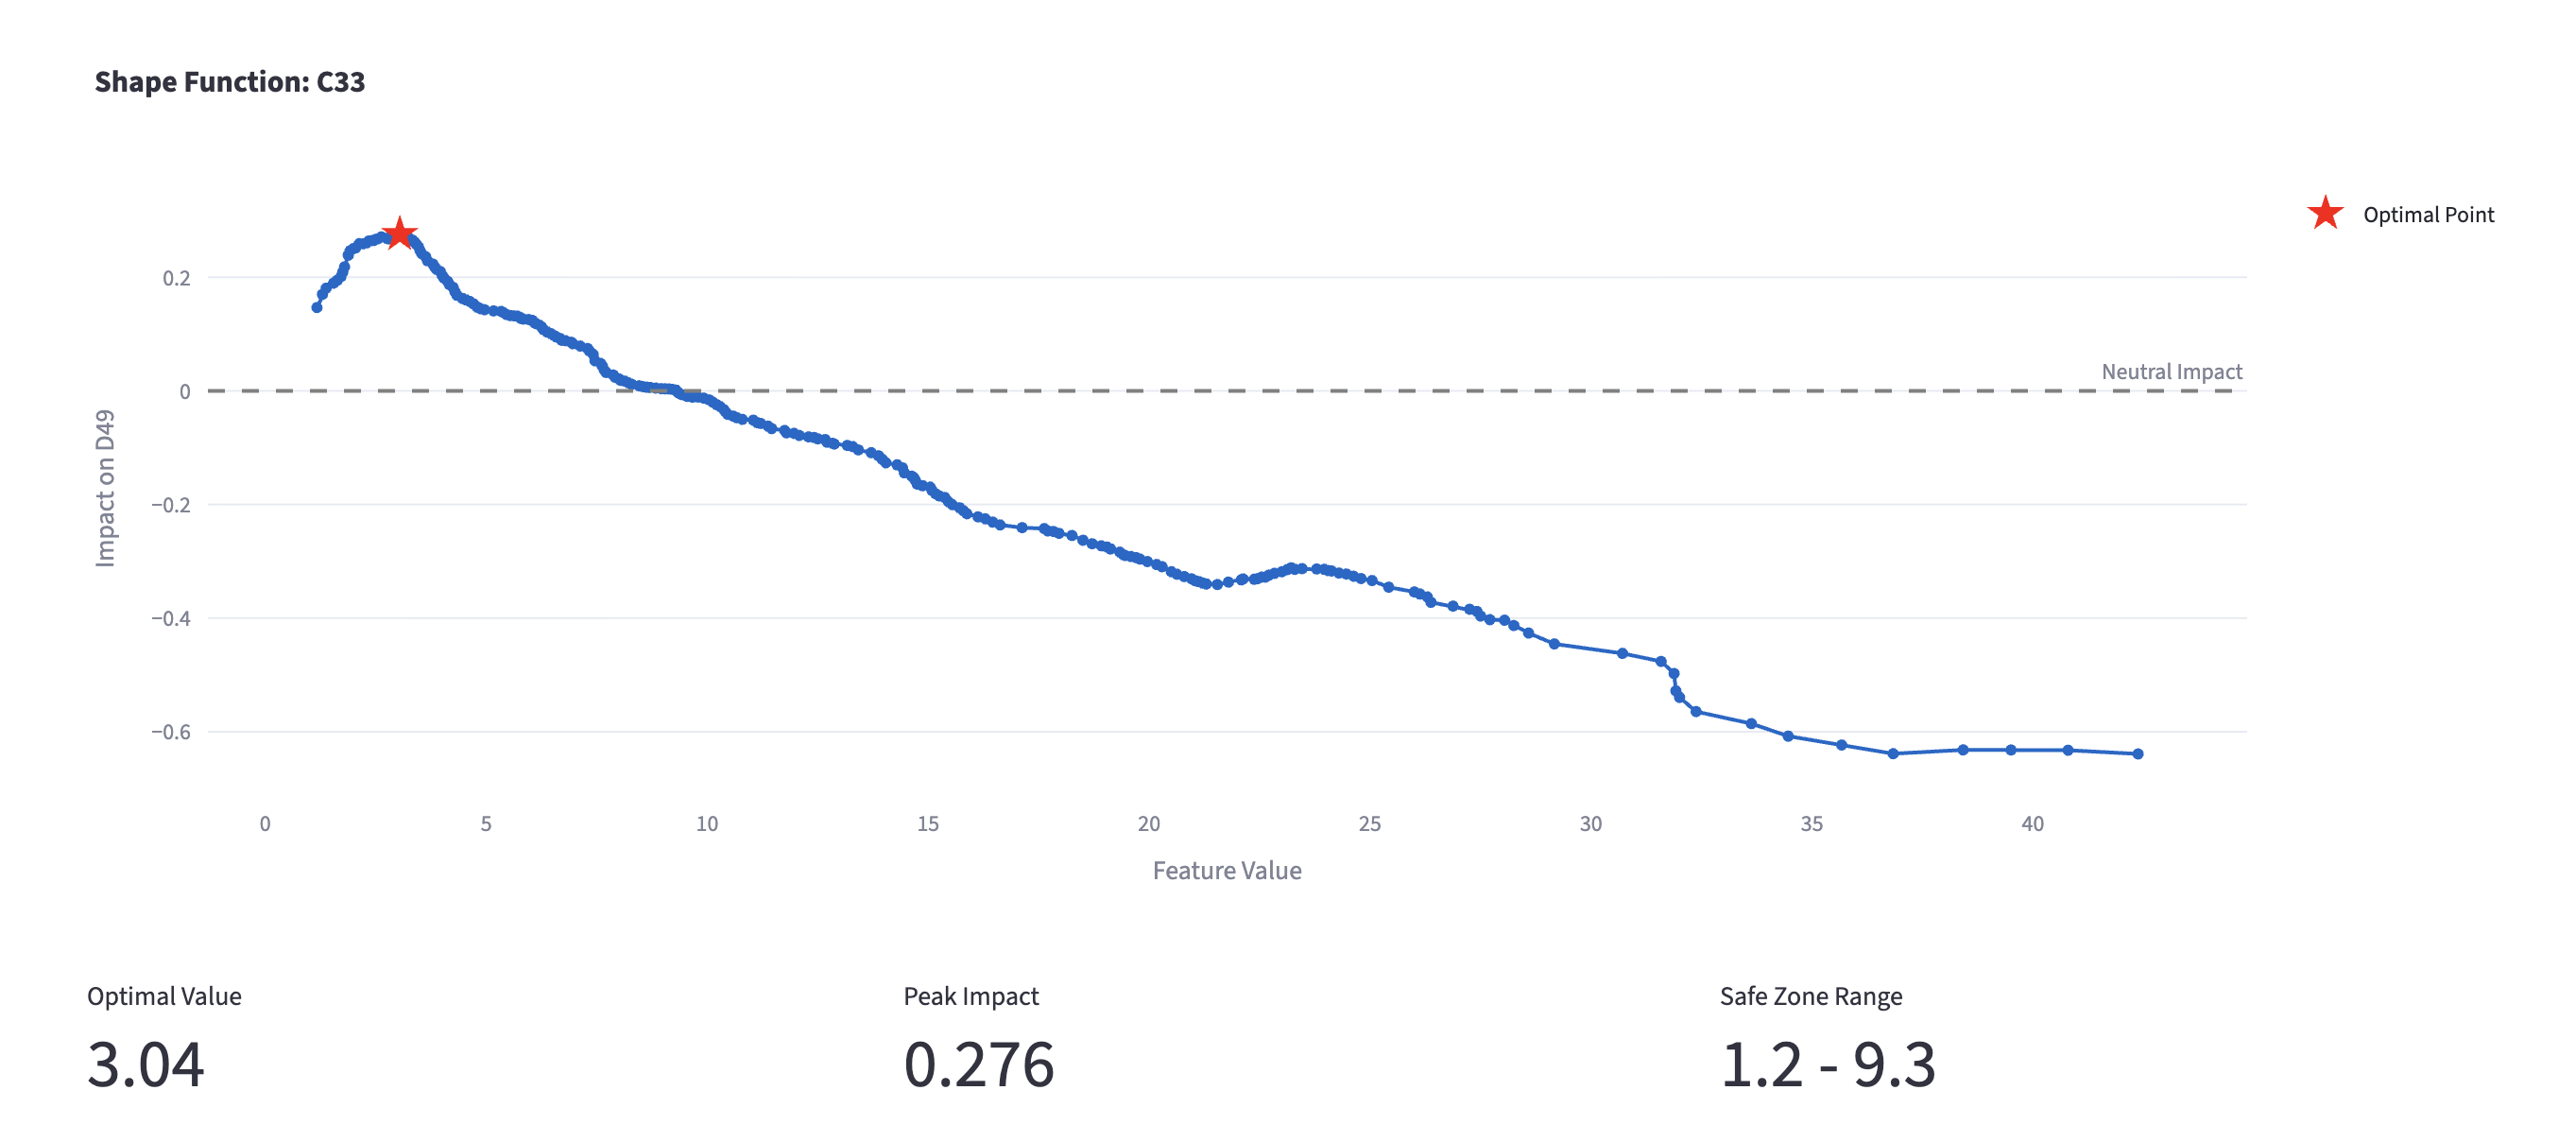
\includegraphics[width=\columnwidth]{images/shape_c33.png}
    \caption{Shape function de C33 (temps total de mescla FI) apresa per l'EBM. La corba mostra la contribució marginal al yield D49: valors propers a 3 minuts maximitzen l'impacte (+0.276 pp), mentre que valors superiors a 10 provoquen penalitzacions creixents fins a $-$0.6 pp. Rang operatiu segur: 1.2--9.3.}
    \label{fig:shape_c33}
\end{figure}

Aquesta informació és directament accionable: un enginyer de procés pot identificar immediatament que el temps de mescla òptim és de 3 minuts, que operar entre 1.2 i 9.3 minuts és segur, i que cada minut addicional per sobre de 10 té un cost quantificable d'aproximadament 0.03~pp de yield — equivalent, al preu de referència de 55~\$/g, a una pèrdua de milers de dòlars per lot. En contrast, l'aproximació \emph{black-box} amb explicabilitat post-hoc (p.~ex. XGBoost + SHAP) presenta tres limitacions fonamentals en aquest context:

\begin{enumerate}
    \item \textbf{Inconsistència entre mètodes post-hoc.} SHAP i LIME poden generar explicacions divergents per a la mateixa predicció, especialment en presència de variables correlacionades \cite{rudin2021fundamental}. L'EBM, en canvi, té una única descomposició exacta per construcció ($f(x) = \beta_0 + \sum_i f_i(x_i) + \sum_{ij} f_{ij}$).

    \item \textbf{Pèrdua d'informació sobre la forma funcional.} SHAP values indiquen la \emph{magnitud} i \emph{direcció} de l'efecte d'una variable per a una observació concreta, però no revelen la \emph{forma} de la relació al llarg de tot el rang. Un enginyer necessita saber no només que ``C33 penalitza en aquest lot'' sinó \emph{per què} (massa curt? massa llarg?) i \emph{quin és el rang òptim}. La shape function de l'EBM respon ambdues preguntes simultàniament.

    \item \textbf{Cost computacional i auditabilitat.} Calcular SHAP values per a un XGBoost amb 2.500 arbres requereix computació significativa per mostra i genera explicacions aproximades. En entorn GxP, on cada explicació ha de ser reproduïble i auditable \cite{gamp5,alcoa}, les aproximacions post-hoc introdueixen un risc de validació addicional que l'EBM evita per disseny.
\end{enumerate}

Des d'una perspectiva operativa, la metodologia redueix l'espai de recerca des del conjunt ampli de variables originals cap a un subconjunt prioritari, facilitant: (1) reducció de complexitat inicial en investigacions RCA; (2) generació d'hipòtesis accionables amb impacte mesurable; (3) traçabilitat de decisions vinculada a evidència quantitativa.

\subsubsection{Impacte operatiu i econòmic del model}

La utilitat de la metodologia proposada rau en la seva capacitat per quantificar el cost d'oportunitat de les desviacions i prioritzar accions de millora basades en evidència quantitativa. Per fonamentar la validesa d'aquestes projeccions, s'ha utilitzat el model configurat com a \textbf{Robust (Leaf=10)}. L'aplicació d'una estratègia de validació creuada de 5 folds suggereix una estabilitat adequada en les mètriques de rendiment (R² = 0.422 i MAE = 0.950 $\pm$ 0.063), redueix el risc de sobreajustament i mostra estabilitat fora de mostra, indicant una capacitat de generalització moderada.

\paragraph{Metodologia d'estimació del potencial optimitzat.} A diferència dels models de caixa negra, l'arquitectura nativament interpretable de l'EBM permet descompondre cada predicció individual com una suma algebraica de contribucions:
\[
f(x) = \beta_0 + \sum_i f_i(x_i) + \sum_{i,j} f_{ij}(x_i,x_j).
\]
Aquesta propietat s'ha utilitzat per identificar, lot a lot, el cost d'oportunitat vinculat a variables operatives subòptimes. El potencial optimitzat de cada lot, $Y_{opt}$, es calcula segons l'expressió següent:
\[
Y_{opt} = Y_{pred} + \left(-Score_{neg} \cdot rec \cdot R^2\right).
\]
On $Score_{neg}$ representa la suma de les contribucions negatives identificades pel model (factors amb impacte inferior a $-0.1$ punts percentuals), i $rec$ és un factor de recuperació operativa fixat en el 70\%. Aquesta penalització del 30\% en la recuperació, sumada a la ponderació per la variància explicada ($R^2=0.422$), constitueix un coeficient de conservadorisme global aproximat del 29.4\%, que integra les limitacions de controlabilitat en planta i les possibles interaccions no lineals no capturades.

Aquest coeficient no és arbitrari, sinó que respon a la integració de dues limitacions fonamentals: (1) \textbf{variància explicada} ($R^2 = 0.422$), que actua com a factor de confiança estadística, assumint que només es pot intervenir sobre la fracció de variabilitat que el model és capaç de capturar; i (2) \textbf{recuperabilitat operativa} ($rec = 0.70$), que aplica una penalització del 30\% per considerar les friccions reals de la planta, com el temps de resposta, la precisió dels equips i les inèrcies del procés. Això reconeix que l'optimització teòrica rarament és assolible al 100\% en entorns GxP. Cal destacar que les contribucions del model s'interpreten com a senyals direccionals associatius, i no com a efectes causals directes sobre el rendiment.

\paragraph{Escenari A: potencial total d'optimització del portfoli.} L'anàlisi de la cartera sobre els lots del període post-canvi revela que la producció presenta oportunitats d'optimització en alguns dels seus paràmetres. En aquest escenari ideal, on es corregirien tots els factors operatius que el model identifica com a \emph{negative drivers}, s'estima un increment del rendiment mitjà (D49) del 46.31\% al 47.32\%. Aquest guany absolut de +1.01 punts percentuals, equivalent a una millora relativa del 2.2\%, suposaria un increment mitjà de facturació de 268.000~\$ per lot produït, assumint un preu de referència de 55~\$/g. En el conjunt del portfoli analitzat, l'oportunitat total ascendeix a 259 milions de dòlars, associats a 4.703 kg de proteïna addicional, amb un impacte recurrent estimat de 26.8 milions de dòlars anuals per a una cadència de 100 lots. Aquest escenari s'ha d'interpretar com un horitzó aspiracional, ja que l'optimització simultània de totes les variables pot veure's limitada per interaccions no lineals o restriccions físiques de la instal·lació.

\paragraph{Escenari B: optimització focalitzada d'alt retorn.} Atès que una intervenció sobre totes les variables pot ser complexa operativament, el model permet identificar una ruta d'optimització simplificada, focalitzada en només tres variables crítiques: D36, paràmetre de filtració que afecta el 62.1\% dels lots; D24, associada a mescla i present en el 50.4\% dels lots; i D40, associada a filtració i present en el 43.0\% dels lots. Aquesta intervenció selectiva permetria capturar de forma immediata un guany de +0.19 punts percentuals de rendiment, aproximadament el 19\% del potencial total del model. Tot i semblar una xifra modesta en termes percentuals, en el context de l'alt valor de la proteïna C activada, aquesta millora focalitzada generaria per si sola uns ingressos addicionals propers als 5 milions de dòlars anuals, justificant la inversió en el sistema de decisió assistida amb un esforç d'ajustament mínim en planta.

\paragraph{Metodologia de càlcul i conservadorisme.} Per garantir la robustesa d'ambdós escenaris davant d'auditories de qualitat, s'ha aplicat un factor de conservadorisme global del 29.4\%. Aquest coeficient no és una agregació lineal de magnituds heterogènies, sinó un filtre en cascada que diferencia la confiança estadística de la viabilitat operativa, seguint principis de prudència en la gestió de riscos en projectes de qualitat biofarmacèutica \cite{rathore2009_qbd}. La confiança del model ($R^2 = 0.422$) actua com a primer tall de prudència, assumint que només és possible intervenir sobre la fracció de variabilitat que el model és capaç d'explicar formalment. La recuperabilitat operativa ($rec=0.70$) aplica una penalització del 30\% per absorbir les inèrcies físiques de la planta i els marges de seguretat GxP, reconeixent que l'òptim teòric és difícilment assolible en la pràctica. Finalment, l'error absolut mitjà (MAE = 0.950) s'utilitza com a referència per filtrar les recomanacions, de manera que el cas de negoci es basi en senyals robustos i no en fluctuacions aleatòries.

Aquesta estructura modular permet justificar que les estimacions no són meres projeccions algorítmiques, sinó un escenari de negoci ajustat a la realitat física i estadística de l'entorn de producció. En aquest sentit, el model actua com un sistema de priorització de decisions operatives basat en evidència, i no com un optimitzador automàtic del procés.

Com a tancament d'aquesta metodologia, i per avaluar la robustesa del cas de negoci davant d'entorns canviants, s'ha analitzat la sensibilitat del projecte davant variacions en les principals hipòtesis econòmiques. Pel que fa al preu base de 55~\$/g, una variació de $\pm$10\% té un impacte proporcional sobre els ingressos estimats, equivalent aproximadament a $\pm$26.800~\$ per lot i $\pm$2.68 milions de dòlars anuals. En tots els casos, el projecte manté una contribució econòmica significativa, indicant una baixa sensibilitat a fluctuacions moderades de mercat. També s'han considerat tres escenaris orientatius d'inversió: un escenari conservador d'aproximadament 1 milió de dòlars anuals, amb retorn altament favorable i immediat; un escenari intermedi d'aproximadament 5 milions de dòlars anuals, en què el cas de negoci continua sent clarament positiu i justificaria per si sol l'estratègia focalitzada de l'Escenari B; i un escenari exigent d'aproximadament 15 milions de dòlars anuals, en què el projecte manté un retorn net positiu, tot i la reducció lògica del marge.

En conjunt, l'anàlisi confirma que el \emph{business case} mostra una robustesa elevada davant les variacions de preu i una sensibilitat moderada al cost d'implementació. Aquest últim és el principal factor de variabilitat en la rendibilitat final, però no compromet la viabilitat financera del projecte.

Un resultat rellevant és que la interpretabilitat s'obté de manera \emph{nativa} amb EBM, no com capa post-hoc. Això implica que les contribucions per variable formen part intrínseca de la predicció, amb descomposició exacta del valor estimat. En comparació amb tècniques post-hoc (SHAP, LIME), l'enfocament natiu redueix inconsistències i simplifica la comunicació amb equips de procés i qualitat \cite{shap_arxiv1705,lime_arxiv1602,rudin2021fundamental}.

\subsection{Comparació amb RCA tradicional i limitacions}

L'enfoc data-driven aporta consistència entre casos, velocitat en priorització i capacitat de tractar múltiples variables simultàniament. Tanmateix, l'RCA tradicional manté fortaleses en profunditat causal contextual i integració de coneixement tàcit. La proposta més robusta és una estratègia \emph{human-in-the-loop}: el model estructura i prioritza l'evidència; l'equip expert valida, contrasta i decideix accions finals. La Figura~\ref{fig:mapa_conceptual} (Apèndix A1) il·lustra esquemàticament ambdós fluxos i el posicionament del sistema ML com a eina de suport dins del procés RCA.

Limitacions identificades: (1) dataset efectiu acotat a 956 mostres; (2) dependència de qualitat de registre; (3) risc de \emph{drift} amb canvis operatius \cite{lu2020drift}; (4) lectura causal limitada per natura observacional; (5) bretxa d'implementació per integració GMP/QMS. El model és un \emph{decision support system}, no substitut de revisió experta.
